%!TEX root = thesis.tex

\chapter{Exploratory Field Study}
\label{chap:exploratory-field-study}

\begin{figure}
\centering
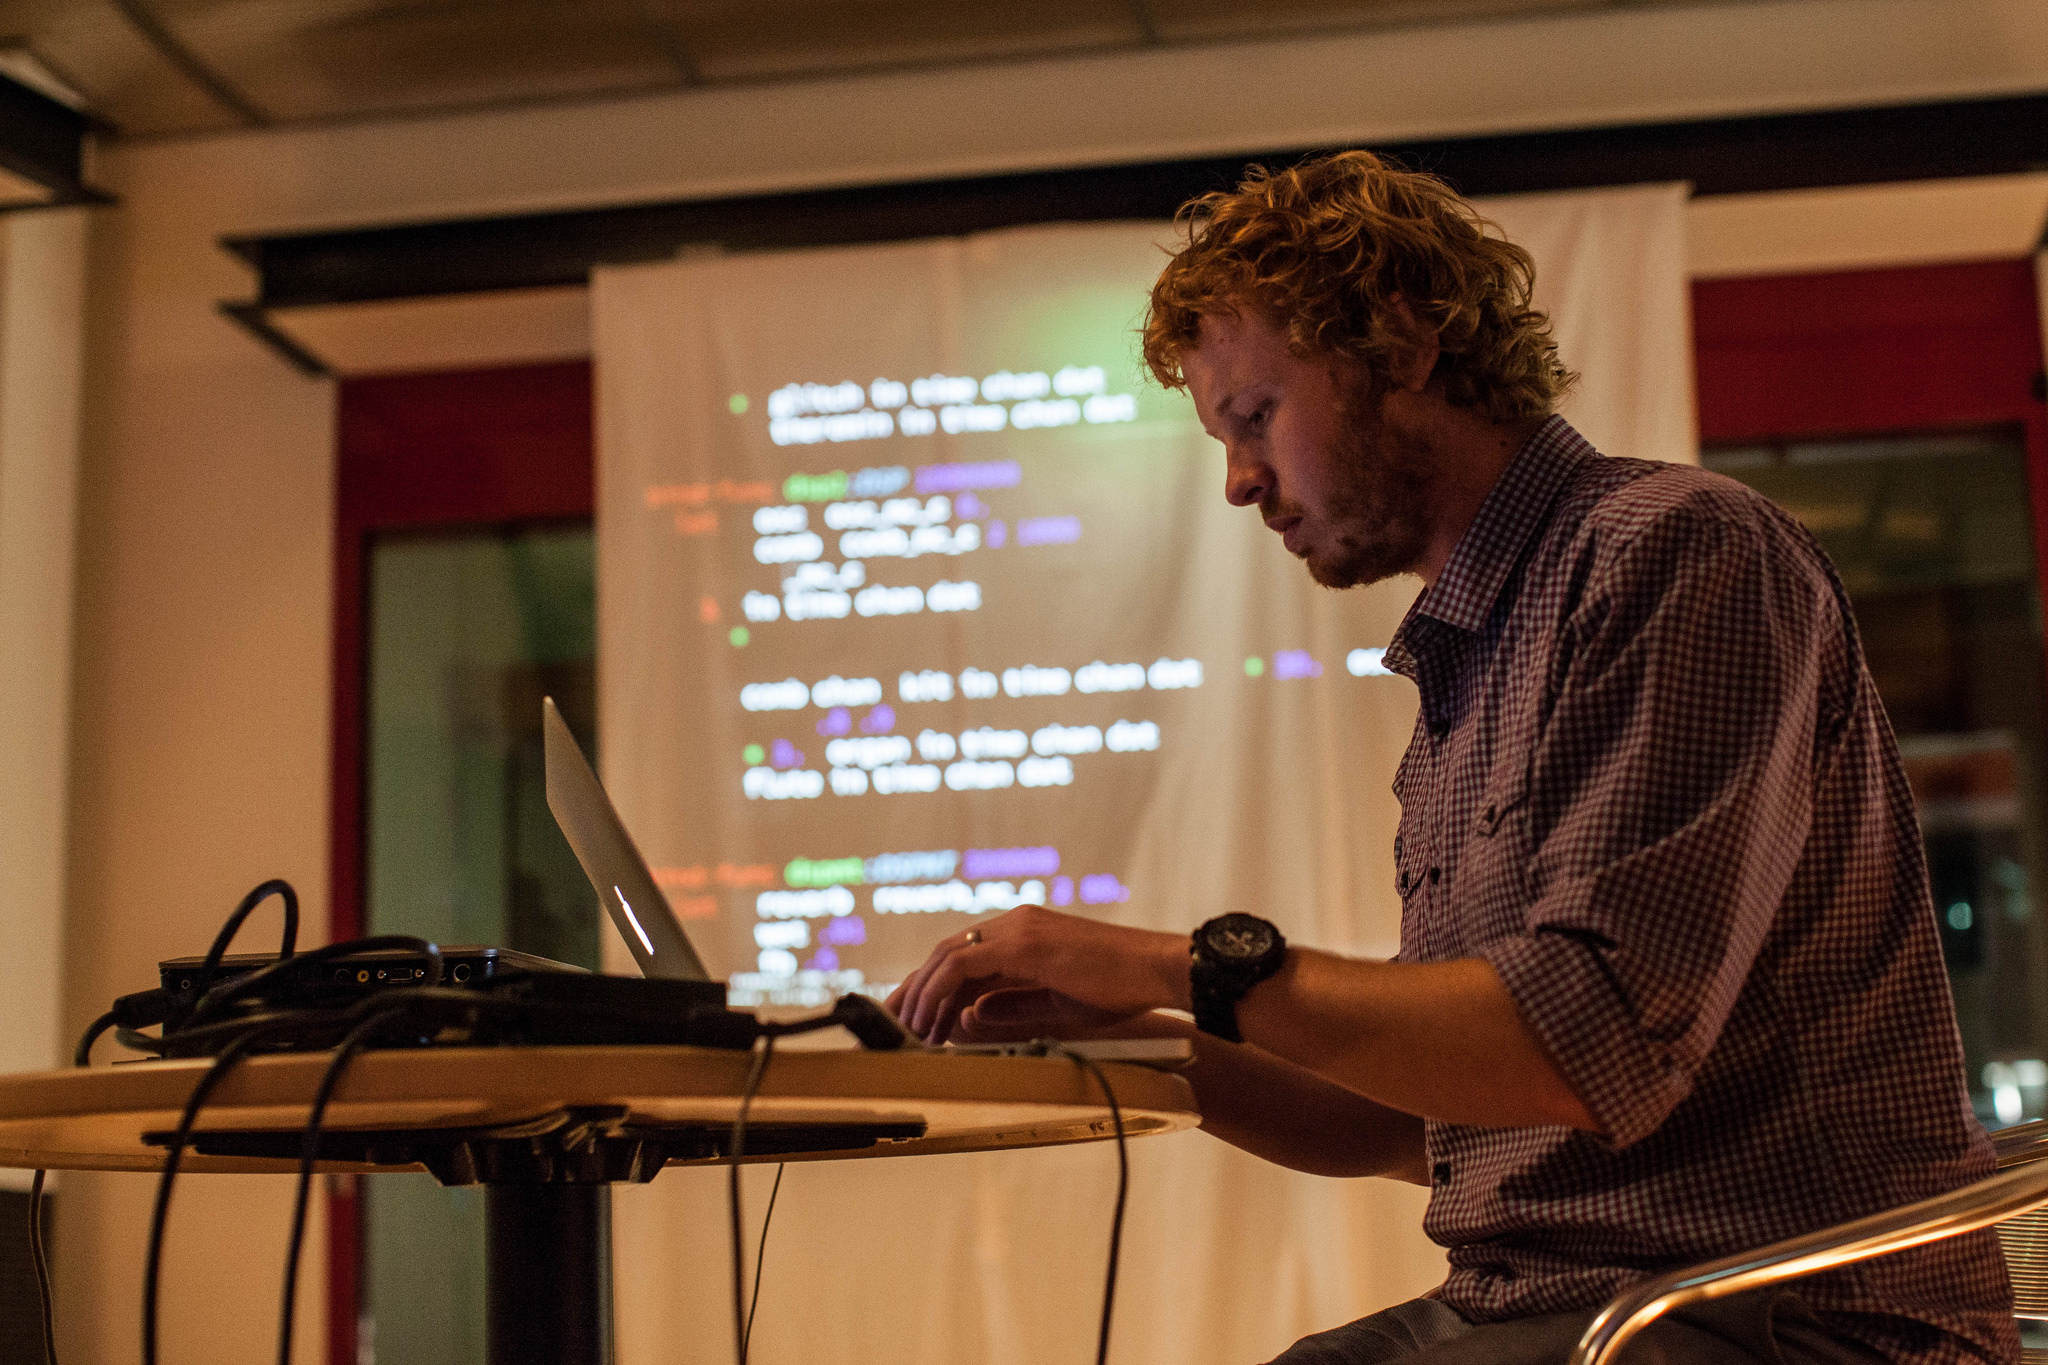
\includegraphics[width=1.0\textwidth]{../images/study-1-you-are-here-ben.jpg}
\caption{A live coder performs at the ``You Are Here'' arts festival in Canberra for an exploratory field study. The standard live coding setup includes a laptop connected to a projector (pictured in foreground) displaying program source code (pictured in background) to an audience.}
\label{fig:exploratory-field-study-ben}
\end{figure}


In order to determine a strategy for visualising source code an exploratory field study was conducted at the ``You Are Here'' arts festival in Canberra. The literature identified the need to re-examine existing models of visualisation and develop a strategy for implementing visualisations within the space of live coding. To this end, an exploratory field study examined the exisiting understanding and enjoyment (as discussed in~\cite{McLean2010a}) of a live coding audience via a survey distributed after a performance. This examined the live coding performance with only the source code projected without any visualiasation. This would provide a baseline for the addition of visualisations to live coding.

In addition to the survey distributed during the performance a set of follow-up email-based interview were conducted. The purpose of these interviews was to gain insight into the audience's current understanding and enjoyment of the live coding process. Additionally, the relationship between enjoyment and understanding was to be examined. It was hoped that the examination of these factors would further inform the development of visualisations targeted at similar audiences and lead to a more general software visualisation strategy.

\section{Method}

Audience members were asked to fill out a survey (see Appendix~\ref{appendix:field-study-survey}) regarding their perception of and response to the projection of the computer code during the performance. Each audience member was asked to indicate which of a number of curves or trajectories best represented their \emph{enjoyment} and \emph{understanding} of the performer's actions in typing the code through the performance. These trajectories allowed for ``high'', ``medium'', and ``low'' levels of enjoyment and understanding for the self-determined ``beginning'', ``middle'' and ``end'' of the performance. Additional questions addressed the audiences sense of ``liveness'' of the performance (c.f.~\cite{Auslander}) and whether the projected code was confusing.
% \begin{itemize}
% \item This was a live performance. What effect did the visuals have on your sense of \emph{liveness} of the performance? \qlab{question:study-1-liveness}
% \item Were there any aspects of the visuals that you found confusing? \qlab{question:study-1-confusion}
% \end{itemize}

Follow-up email questions were distributed following the performance to a number of those in attendance. The follow-up email asked two questions: 
\begin{itemize}
\item What did you \emph{understand} about what was going on with the code being projected? In particular, what did you understand about the relationship between the code and the music? \qlab{question:study-1-email-understand-relationship}
\item Would would you like to understand more about the code in order to enjoy the performance more? \qlab{question:study-1-email-understand-enjoy}
\end{itemize}

\section{Participants}

A total of thirteen survey responses were received. Of these, 77\% regularly listen to music and 54\% perform regularly. 38\% of the respondents stated that they had high exposure to programming through work, study or their hobbies, 31\% stated that they had some experience and 31\% stated that they had no experience with it. Of the respondents, 69\% had never been to a live coding performance before.

77\% stated that they listen to large amounts of music compared to 23\% that stated they only listened to a small amount. 54\% stated that they performed music reguarly, 16\% stated that they performed only occasionally while 31\% stated that they had never performed music.

\section{Results}

\subsection{Survey}

Of the thirteen survey responses received, six audience members showed a high level of enjoyment throughout the whole performance, while the remaining seven responses showed alternating levels of enjoyment. No audience members indicated a low level of enjoyment throughout the performance.  Only two of the thirteen respondents indicated that they understood the relationship between the code projections and the music throughout the performance. Three of the six respondents who reported a high level of enjoyment throughout the performance also indicated an increase in understanding (from low to high) as the performance progressed, although a Chi-square analysis revealed no significant relationship between enjoyment and understanding due to the small sample size. 

When asked if the projected code helped to communicate a sense of liveness, nine members of the audience indicated that the projected code helped whereas four members of the audience indicated that the projected code had no effect on their sense of liveness.

Regarding confusion, five members of the audience stated that they found no aspects of the visuals confusing. For the members of the audience that stated confusing aspects of the performance, aspects identified as confusing included the small font, the difficulty linking changes in the source code to changes in the sound and the flicking between screens. Four members of the audience did not respond to the question.

\subsection{Follow-up Interview}

The follow-up interview identified some gaps in understanding from the survey. A total of three email responses were received. When asked what these audience members felt they understood about the performance (see Question~\ref{question:study-1-email-understand-relationship}), all three responses indicated high understanding of the intial process of building the music from scratch and developing the musical forms to be modified throughout the performance. One of the responses indicated that they could see changes being made but could not identify which elements within the source code related to which elements in the music. Notably, one audience member stated that they didn't ``have a big picture of what all the code looks like'' and this caused them difficulty in understanding the live coding process. 

The second follow-up interview question asked what should be made clearer within the space of live coding (see Question~\ref{question:study-1-email-understand-enjoy}) prompting a variety of responses. Two audience members stated that more understanding of the ideas or source code changes would be desirable. However, one of the responses indicated that a higher understanding of the live coding performance may result in lower enjoyment, taking focus away from the enjoyable parts of the performance but noted that it may be due to their background and those with less experience in music or programming may find a higher understanding more beneficial.

Results of the follow-up email interview are available in Appendix~\ref{appendix:field-study-follow-up-interviews}.

\section{Discussion}

Despite the small sample size, a large proportion of the audience indicated that the code was confusing to those with little previous experience. This confusion was confirmed within the follow-up interviews. Despite this confusion, the projected code still conveyed that the programmer was modifying the music, the positive contribution to liveness identified by 70\% of the audience. This was also confirmed within the follow-up interviews in which the interviewees indicated that during the early stages of the performance, the relationship between writing the code and triggering the music was clear.

\more
% -various things made the performance confusing

A minority of the audience stated that they found the source code projections confusing and only a very small number of respondents claimed to have actually understood what the programmer was doing. We were quite intrigued by the small cohort of respondents whose understanding increased through the performance and whose enjoyment remained high, and we wished to test whether augmenting code projections with additional visualisations might increase the understanding and enjoyment of the audience in live coding. \fix

\subsection{Validity}

Due to the layout of the venue, in some locations the projection screen may have been difficult to see. Additionally, the projection screen surface was uneven and due to the projector contrast the projected source code, particularly the punctuation, was difficult to see. This may have contributed to confusion among those with some background in programming.

\more

\subsection{Limitations}

Results of this study were constrained by sample size. Although the follow-up interview identified some interesting problems within the current live coding practice, it was determined that more could be gained from surveying a larger audience.

In addition, the survey was found to be too limited to make more than basic judgements regarding the audience reported understanding and enjoyment. The six multiple choice options provided did not allow for evaluation of specific sections of the performance regarding the dimensions.

\section{Summary}

This study identifies the need to reduce confusion within the space of live coding. Understanding during the early stages of the performance was shown to be high within the interviews but drifted as more code was added. Modifications during the middle and end of the performance were apparent to the audience but their intention was not clear.

Taken as a whole, the results of this small field study were salutatory towards the benefit of ``seeing as well as hearing'' code during a live coding performance, especially as far as the general public is concerned. \fix

This exploratory field study identified some...\more


